\section{改进策略}\label{sec-4}
\subsection{非线性激活函数的选取}\label{sec-4:nonlinear-activation}
本策略来自论文\textit{GLU Variants Improve Transformer}\citep{shazeerGLUVariantsImprove2020}。

Transformer模型通过多头注意力层和FFN层交替工作。FFN层存在于Transformer架构的编码器和解码器部分中。这个网络的结构是:
    $$
    \text{FFN}(x, W_1, W_2, b_1, b_2) = \max(0, xW_1 + b_1)W_2 + b_2
    $$
    其中,$ x $ 是输入,$ W_1 $ 和 $ W_2 $ 是权重矩阵,$ b_1 $ 和 $ b_2 $ 是偏置向量。
    
    这个公式首先通过一个线性变换 $ xW_1 + b_1 $,然后通过 ReLU 激活函数,最后再通过另一个线性变换 $ W_2 $ 和偏置 $ b_2 $。
    
    在本文中,作者对前馈网络进行了一些调整,取消了偏置项。这样做的目的是为了简化模型和提高训练效率。调整后的前馈网络结构是:
    $$
    \text{FFN}_{\text{ReLU}}(x, W_1, W_2) = \max(0, xW_1)W_2
    $$
    这个公式中,去掉了偏置项 $ b_1 $ 和 $ b_2 $,只保留了 ReLU 激活函数和两个权重矩阵。
    
    除了 ReLU 激活函数,还有一些其他的激活函数被用于前馈网络中。例如,基于高斯误差函数的激活函数 GELU 可以用于前馈网络,其结构是:
    $$
    \text{FFN}_{\text{GELU}}(x, W_1, W_2) = \text{GELU}(xW_1)W_2
    $$
    GELU 激活函数可以更好地模拟神经网络的随机正则化行为,从而提高模型的性能。
    
    另一个被用于前馈网络的激活函数是 Swish。Swish 激活函数是一个自门控的激活函数,它可以自动调节每个神经元的输出。基于 Swish 激活函数的前馈网络结构是:
    $$
    \text{FFN}_{\text{Swish}}(x, W_1, W_2) = \text{Swish}(xW_1)W_2
    $$
    Swish 激活函数在某些情况下可以提高神经网络的性能,因此在设计前馈网络时,可以根据具体的应用场景选择合适的激活函数。
\subsubsection{门控线性单元(GLU)及其变种}
    在神经网络中,门控线性单元(GLU)作为一种有效的激活机制被广泛应用。其核心思想是通过引入一个门控机制来调节信息流动,从而增强模型的表达能力。GLU 的数学表达式为:
    $$
    \text{GLU}(x, W, V, b, c) = \sigma(xW + b) \otimes (xV + c)
    $$
    这里,$ x $ 表示输入向量,$ W $ 和 $ V $ 是权重矩阵,而 $ b $ 和 $ c $ 分别是偏置项。符号 $ \sigma $ 表示sigmoid激活函数,$ \otimes $ 表示逐元素乘法。
    
    进一步简化 GLU 模型,如果去掉激活函数 $ \sigma $,则得到一种称为 Bilinear 的变体,其公式为:
    $$
    \text{Bilinear}(x, W, V, b, c) = (xW + b) \otimes (xV + c)
    $$
    
    在此基础上,研究者们提出了几种基于不同激活函数的 GLU 变体,以探索更优的性能表现:
    \begin{itemize}
    	\item \textbf{ReGLU}:使用ReLU激活函数替代sigmoid:
    	$$
    	\text{ReGLU}(x, W, V, b, c) = \max(0, xW + b) \otimes (xV + c)
    	$$
    	
    	\item \textbf{GEGLU}:则采用GELU作为激活函数:
    	$$
    	\text{GEGLU}(x, W, V, b, c) = \text{GELU}(xW + b) \otimes (xV + c)
    	$$
    	
    	\item \textbf{SwiGLU}:引入了参数化的 Swish 激活函数,其中 $ \beta $ 是可学习的参数:
    	$$
    	\text{SwiGLU}(x, W, V, b, c, \beta) = \text{Swish}_\beta(xW + b) \otimes (xV + c)
    	$$
    \end{itemize}
    
    接下来,我们考虑将上述激活函数应用于前馈神经网络(FFN),构建了一系列新的 FFN 结构:
    $$
    \text{FFN}_{\text{GLU}}(x, W, V, W_2) = (\sigma(xW) \otimes xV) W_2
    $$
    $$
    \text{FFN}_{\text{Bilinear}}(x, W, V, W_2) = (xW \otimes xV) W_2
    $$
    $$
    \text{FFN}_{\text{ReGLU}}(x, W, V, W_2) = (\max(0, xW) \otimes xV) W_2
    $$
    $$
    \text{FFN}_{\text{GEGLU}}(x, W, V, W_2) = (\text{GELU}(xW) \otimes xV) W_2
    $$
    $$
    \text{FFN}_{\text{SwiGLU}}(x, W, V, W_2) = (\text{Swish}_1(xW) \otimes xV) W_2
    $$
\subsubsection{模型评估}
\noindent\textbf{翻译任务实验}

    作者使用基于Transformer架构的T5模型在文本翻译任务上进行实验,比较了不同激活函数变体在65,536次和524,288次训练步骤后的log-perplexity表现。
    
    实验结果表\ref{tab:results}表明,GEGLU和SwiGLU变体在这两个训练阶段都取得了最低的困惑度(perplexity),这说明它们在提高翻译质量方面具有显著的优势。
    
    
\noindent\textbf{语言理解任务实验}

    为了进一步验证这些变体的有效性,作者在GLUE(General Language Understanding Evaluation)基准测试上进行了实验。
    
    结果表\ref{tab:glue_results1}显示,在多个子任务中,SwiGLU、ReGLU 和 Bilinear 变体均表现出色,至少在三个不同的任务上达到了最优或接近最优的结果。这一发现证明了这些变体在语言理解任务中的有效性。
    
    此外,作者还探讨了使用预训练模型进行去噪,并随后在下游任务中应用不同激活函数的效果。
    
    实验表\ref{tab:glue_results2}表明,在基于预训练-微调的语言理解任务中,GEGLU、Bilinear 和 SwiGLU 变体同样展示了优异的表现,分别在多个任务上取得了最佳成绩。这些结果支持了假设,即这些激活函数变体不仅能增强模型的表现力,还能促进模型从大规模预训练数据中更有效地迁移知识到特定任务中。
    
    
    综合以上实验结果,作者提出相应建议:
    \begin{itemize}
    	\item \textbf{翻译任务:}鉴于GEGLU和SwiGLU在翻译任务上的出色表现,我们推荐在未来的翻译模型设计中优先考虑这两种激活函数变体。
    	\item \textbf{语言理解任务:}对于语言理解任务,尤其是涉及复杂语义分析的任务,SwiGUE、ReGLUE 和 Bilinear 是值得尝试的选择,因为它们能够提供更好的表达能力和泛化性能。
    	\item \textbf{预训练-微调框架:}在采用预训练-微调框架处理语言理解任务时,GEGLU、Bilinear 和 SwiGLU 的组合可能是提升模型性能的有效策略。
    \end{itemize}
\subsection{LN结构调整}\label{sec-4:ln-adjust}
本策略来自论文\textit{On Layer Normalization in the Transformer Architecture}\citep{xiongLayerNormalizationTransformer2020}。

该文研究了Transformer架构中层归一化(Layer Normalization)的位置对模型训练稳定性的影响,一共进行了三次实验。在传统的Transformer中,层归一化位于残差块之间(称其为Post-LN),这会导致在初始化时输出层附近的参数梯度较大。使用较大的学习率会导致训练不稳定。如图\ref{fig:layer-structure}.

\begin{figure}[ht]
    \centering
    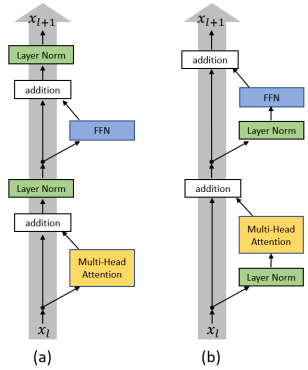
\includegraphics[height=7cm]{img/LN/LN-1.jpg}
    \caption{(a) Post-LN Transformer layer; (b) Pre-LN Transformer layer.}
    \label{fig:layer-structure}
\end{figure}

同时为了验证其性能,该文同时验证了学习率预热阶段的依赖性:为了稳定训练,通常需要一个精心设计的学习率预热阶段。这个阶段虽然对最终性能至关重要,但会减慢优化过程并增加超参数调整的复杂性。以上为该文的两个主要贡献。

\subsubsection{warm-up机制}

首先我们需要了解什么是warm-up。在优化Transformer结构时,除了像训练一般模型一样设置初始学习率与它的衰减策略(Adam,SGD),往往还需要在训练的初始阶段设置一个非常小(接近0)的学习率,让它经过一定的迭代轮数后逐渐增长到初始的学习率,这个过程也被称作warm-up阶段。

warm-up是原始Transformer结构优化时的一个必备学习率调整策略。Transformer结构对于warm-up的超参数(持续轮数、增长方式、初始学习率等)非常敏感,若调整不慎,往往会使得模型无法正常收敛。

该文在IWSLT14 De-En翻译数据集上使用Transformer模型对warm-up的效果进行验证,采用Adam和SGD两种随机优化器,分别测试了两种学习率($1 \times 10^{-3}$, $5 \times 10^{-4}$)在没有warm-up(0轮), warm-up迭代轮数不足(500轮)和迭代轮数充足(4000轮)情况下模型的验证集Loss与BLEU分数,结果如图\ref{fig:performance}所示。

\begin{figure}[ht]
    \centering
    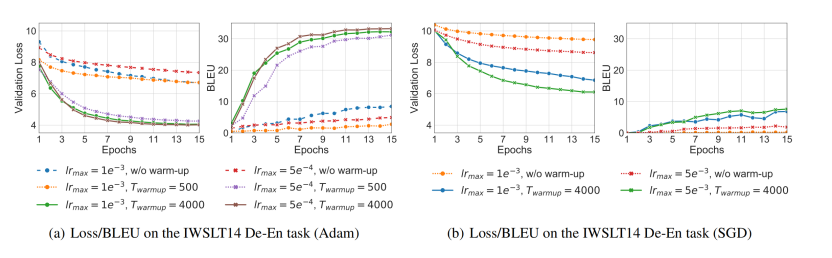
\includegraphics[width=\textwidth]{img/LN/LN-2.jpg}
    \caption{Performances of the models optimized by Adam and SGD on the IWSLT14 De-En task.}
    \label{fig:performance}
\end{figure}

从实验中可以看出,模型最终性能对无论是warm-up所需迭代轮数还是学习率的大小都非常敏感,由于Transformer优化困难的阶段是在训练的初始阶段,warm-up也只是在迭代的前若干轮起作用,因此从模型的初始化阶段开始探究原因。

\subsubsection{LN执行对对梯度范数的影响}

Transformer层的初始化方式通常是Xavier方法,通过对各隐层梯度值进行分析可以证明,在初始化点附近的Post-LN Transformer结构最后一层的梯度值非常大,同时随着反向传播的前传会导致梯度值迅速衰减。这种在各层之间不稳定的梯度分布必然会影响优化器的收敛效果,导致训练过程初始阶段的不稳定。造成Post-LN Transformer梯度分布出现问题的核心原因在于各子层之后的Layer Normalization层会使得各层的输入尺度与层数\(L\)无关,因此当Layer Normalization对梯度进行归一化时,也与层数\(L\)无关。

作者提出Pre-LN Transformer,即将层归一化放在残差块内部,在每个子层(如自注意力机制或前馈神经网络)之后进行归一化,而不是在残差连接之后,并且在整个网络最后输出之前也增加一个Layer Normalization层来对梯度进行归一化。

使用相同的方法对Pre-LN Transformer结构进行分析后,发现最后一层Layer Normalization层的输入尺寸的量级只有Post-LN的\(\sqrt{1/L}\)倍,并且每个LN层都会对梯度以\(\sqrt{L}\)的比例归一化。所以对于Pre-LN结构来说,其每层梯度范数都近似不变。

该文在IWSLT 14 De-En数据集对两种结构在初始化附近以及经过了warm-up阶段的梯度范数进行了实验验证,结果如图\ref{fig:gradients}所示。
\begin{figure}[h]
    \centering
    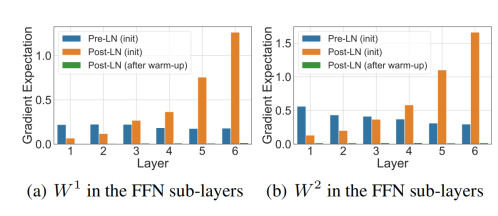
\includegraphics[width=11cm]{img/LN/LN-3.jpg}
    \caption{The norm of gradients of different layers in the Transformer.}
    \label{fig:gradients}
\end{figure}

可以看出,相比于Post-LN结构梯度分布的不稳定,Pre-LN在各层之间梯度范数几乎保持不变,这种结构明显更利于优化器进行优化。而在进行一定轮数的warm-up后,Post-LN的梯度范数也基本保持不变,并且其量级非常小,这也验证了理论。

\subsubsection{模型评估}

最后,在IWSLT、WMT和BERT三个任务上实验验证了是否可以在Pre-LN结构中去掉warm-up,结果如图\ref{fig:iwslt-wmt5}、\ref{fig:bert}所示。
\begin{figure}[h]
    \centering
    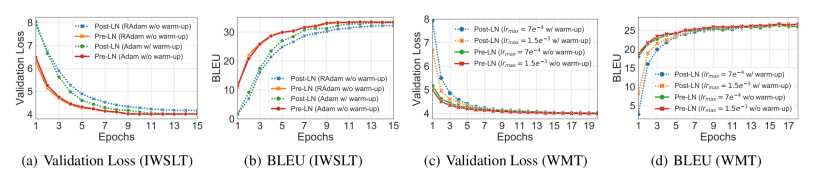
\includegraphics[width=\textwidth]{img/LN/LN-4.jpg}
    \caption{Performances of the models on the IWSLT14 De-En task and WMT14 En-De task.}
    \label{fig:iwslt-wmt5}
\end{figure}

\begin{figure}[ht]
    \centering
    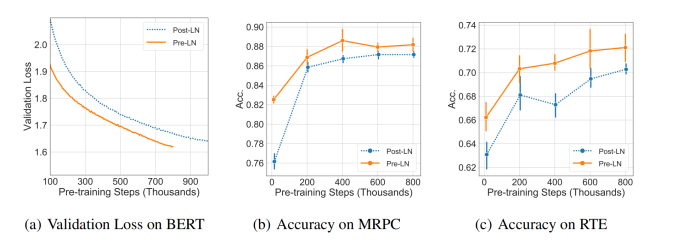
\includegraphics[width=14cm]{img/LN/LN-5.jpg}
    \caption{Performances of the models on unsupervised pre-training (BERT) and downstream tasks.}
    \label{fig:bert}
\end{figure}

实验结果表明,当使用Pre-LN结构时,warm-up阶段已经不再是必需,并且Pre-LN结构可以大幅提升Transformer的收敛速度。对于机器翻译任务(IWSLT/WMT),不需要warm-up的Pre-LN结构可以比Post-LN收敛快1倍左右,而在BERT上,Pre-LN在下游任务上达到和Post-LN相同的性能也只需要后者迭代轮数的1/3左右,并且最终的效果也更好。

总之,Pre-LN Transformer在没有学习率预热阶段的情况下,可以在多种应用中达到与Baseline相当的结果,同时显著减少了训练时间和超参数调整。

\subsection{相对位置编码}\label{sec-4:rel-pos-encoding}
本策略来自论文\textit{Self-Attention with Relative Position Representations}\citep{shawSelfAttentionRelativePosition2018}。

Transformer的架构Self-Attention机制本质上是无序的,即它对输入序列的排列顺序不敏感,这导致原始Transformer模型难以直接捕捉到token之间的相对或绝对位置信息。为了解决这个问题,通常的做法是在输入嵌入中加入位置编码(Positional Encoding),以此间接地向模型提供序列元素的位置信息。

本文提出了一种方法,通过改进Self-Attention机制,在其内部直接整合token间的相对位置关系向量,从而打破了原有的排列不变性,使得Self-Attention不仅能够感知到序列中元素的位置,而且更高效地编码这些位置信息,无需依赖外部附加的位置特征。
\subsubsection{关系感知自注意力机制}
考虑一个有向全连接图,其节点由输入元素构成,并且每条从$x_i$指向$x_j$的边都附带有一对向量$\alpha_{ij}^V, \alpha_{ij}^K \in \mathbb{R}^{d_\alpha}$作为特征描述,这里$d_a = d_z$。这些向量在所有注意力头中共享,以捕捉节点间的相对位置信息。通过引入边的特性表示,传统的自我注意(Self-Attention)机制被重新定义为如下形式:
\begin{align*}
    z_i &= \sum_{j=1}^{n} \alpha_{ij} \left( x_j W^V + \alpha_{ij}^V \right)\\
    \alpha_{ij} &= \frac{\exp e_{ij}}{\overunderset{n}{k=1}{\sum}\exp e_{ik}}\\
    e_{ij} &= \frac{x_i W^Q \left( x_j W^K + \alpha_{ij}^K \right)^T}{\sqrt{d_z}}
\end{align*}
其中,每个Value ($T^V$) 和 Key ($T^K$) 都附加了位置关系编码,从而使得该注意机制不再对节点顺序保持不变。
\subsubsection{相对位置编码}
鉴于计算复杂度、内存占用以及远距离精确位置信息的边际效益递减等因素,本文中对相对位置距离施加了最大限制$k$。具体而言,当节点间的实际距离超出这一界限时,我们将它们的位置差异截断至这一范围内。这可以形式化为:
\begin{align*}
    a_{ij}^K &= w_{\text{clip}(j-i, k)}^K\\
    a_{ij}^V &= w_{\text{clip}(j-i, k)}^V\\
    \text{clip}(x, k) &= \max(-k, \min(k, x))
\end{align*}
其中,$\text{clip}$函数确保任何一对节点之间的相对位置编码不会超过预设的最大距离$k$。在这种情况下,模型只需要学习有限集合的参数:对于Key ($\omega^K = (\omega_{-k}^K, \ldots, \omega_k^K)$) 和 Value ($\omega^V = (\omega_{-k}^V, \ldots, \omega_k^V)$),每个方向各有$k$个不同的位置权重。
\subsubsection{高效实现}
引入相对位置编码后,作者将原本的键值$k_{ij}$分解成两个独立的部分,以便分别进行高效的矩阵运算。这使得每个部分都可以通过并行计算加速,具体公式如下:
$$
e_{ij} = \frac{x_i W^Q \left( x_j W^K \right)^T + x_i W^Q \left( a_{ij}^K \right)^T}{\sqrt{d_z}}
$$
其中,第一项与未添加相对位置编码时的计算方法相同,而第二项则利用了位置编码$b_{ij}^K$进行了调整。设上式右侧为$e'_{ij}$,令$x_i W^Q = q_i$,并且$a_{ij}^K = k_{ij}$,忽略分母,则有$e'_{ij} = q_i k_{ij}^T$。

在这样的设置下:
\begin{itemize}
\item 我们拥有$bh \times n$个$q_i$,每个$q_i$的维度是$d_z$。
\item 同样地,存在$n \times n$个$k_{ij}$,每个$k_{ij}$的维度也是$d_z$。
\end{itemize}

为了实现高效矩阵运算,需要对$q_i$和$k_{ij}$进行重新组织:
\begin{itemize}
\item $q_i$可以被视作$n \times bh$个$q'_i$,每个$q'_i$仍具有$d_z$的维度。
\item 对于$k_{ij}$,它同样可以被看作$n \times n$个$k'_{ij}$,每个$k'_{ij}$保持$d_z$的维度不变。
\end{itemize}

这样一来,我们可以针对$q'_i$和$k'_{ij}$执行$n$次并行的矩阵乘法操作,每次涉及两个大小分别为$bh \times d_z$和$d_z \times n$的矩阵。完成这些计算之后,再将结果重新组织回原来的形状,以完成$e_{ij}$两部分的高效并行化计算。

此时我们便可以对$q'_i$和$k'_{ij}$进行$n$个并行化的两个大小为$bh \times d_z$和$d_z \times n$的矩阵计算来加速计算。最终再重新reshape回原始的大小即可完成$e_{ij}$两个部分的高效并行化计算。
\subsubsection{模型评估}
本篇论文主要是用于NLP领域,使用newstest2014测试集,WMT 2014英语到德语(EN-DE)和英语到法语(EN-FR)翻译任务,其实验结果如表\ref{tab:results1},\ref{tab:clipping-distance-results},\ref{tab:ablation-results}。

总的来说,本文提出了一种扩展自注意力机制的方法,该方法能够有效地将序列元素间的相对位置信息融入到模型中,从而提升了机器翻译任务的性能。通过这种改进,模型可以在不依赖显式的位置编码(即硬位置编码)的情况下处理位置信息。

不过论文中并未直接对比新方法与传统硬位置编码在效果上的差异。


\subsection{稀疏注意力机制}\label{sec-4:sparse-attention}
本策略来自论文\textit{Generating Long Sequences with Sparse Transformers}\citep{childGeneratingLongSequences2019}。

Transformer最被诟病的一个问题是它的时间复杂度以及空间复杂度和输入序列的长度成二次方的关系$O(n^2)$。而这篇文章提出的Sparse Transformer方法使用稀疏自注意力替代了传统Transformer的密集自注意力,将Transformer的复杂度降低到$O(n^{3/2})$。

在CIFAR-10数据集上,使用一个128层的自注意力模型。对注意力进行可视化,得到图\ref{fig:iwslt-wmt1}:

\begin{figure}[h]
    \centering
    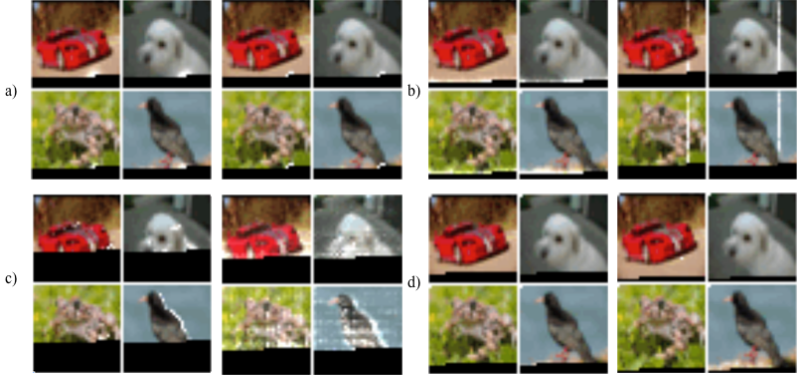
\includegraphics[width=\textwidth]{img/SC/SC1.jpg}
    \caption{Learned attention patterns from a 128-layer network on CIFAR-10 trained with full attention.}
    \label{fig:iwslt-wmt1}
\end{figure}

白色区域是注意力机制的高权值位置,黑色区域是被mask掉的位置,从a到d为层数逐渐加深的过程,可以看到注意力头的权重分布从浅至深呈现出“周围——行列——全局——全局稀疏”的变化过程。那么直接在注意力头上利用这种稀疏性是否可以加速计算,这需要一系列设计和验证。

\subsubsection{连接模式}

像GPT这样的自回归模型,使用的是之前所有时间片的内容来预测当前时间片的结果。传统的Transformer需要为之前的所有时间片计算一个权值,所以传统Transformer的自注意力机制的复杂度是$O(n^2)$。如下图\ref{fig:iwslt-wmt2}(a)中为大小$6\times6$图像的注意力和长度为16的注意力连接矩阵。

\begin{figure}[h]
    \centering
    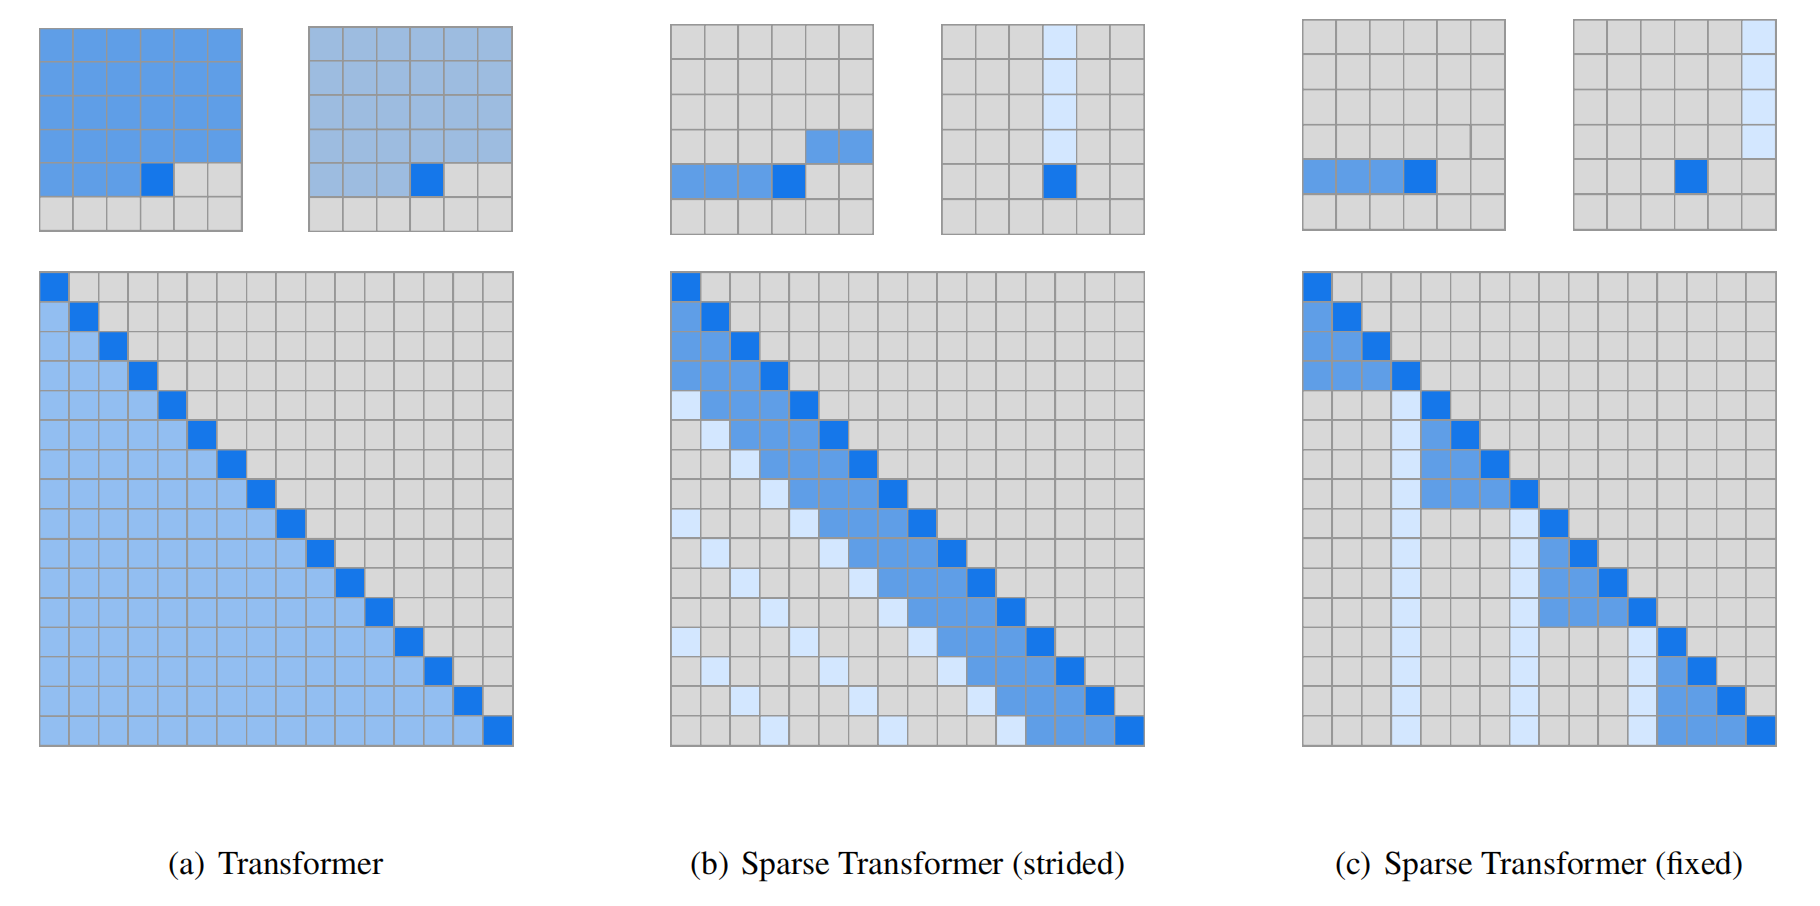
\includegraphics[width=\textwidth]{img/SC/SC2.jpg}
    \caption{Two 2d factorized attention schemes we evaluated in comparison to the full attention of a standard Transformer (a).}
    \label{fig:iwslt-wmt2}
\end{figure}

传统的自注意力的计算方式可以表示为:
\[
\text{Attention}(Q, K, V) = \text{softmax}\left(\frac{QK^T}{\sqrt{d_k}}\right)V
\]

该计算方式复杂度最高的地方是$QK^T$,而Sparse Transformer的核心是只让设置好的像素点参与自注意力的计算。这里不是只选取设置好位置上的像素点,其他mask掉,因为这样并不能降低模型的复杂度。

为了实现上述目标,我们这里引入一个名为连接模式(Connectivity Pattern)的变量,它表示为$S = \{S_1, S_2, \ldots, S_n\}$,其中$S_i$表示预测第$i$个时间片的索引。形象地说,它可以表示为一个由0和1组成的二维矩阵,二维矩阵中的数值为1表示该位置的像素点参与自注意力的计算。如在上图中,位置为28,则传统自注意力中$6\times6$大小$S_{28}$的表示为(a)的上半部分,其中深色部分为1,浅色部分为0。

在Sparse Transformer的自注意力计算中,连接模式只作用在$K$和$V$的计算上,计算过程如下所示。

1. 对于第 \(i\) 个时间片的输入,首先使用 \( \text{key} \) 和 \( \text{value} \) 的权值矩阵乘以输入特征,得到 \( K \) 和 \( V \)。然后再将连接模式 \( S_i \) 作用到 \( K \) 和 \( V \) 上,得到稀疏的特征 \( K_{S_i} \) 和 \( V_{S_i} \)。
   \[
   K_{S_i} = (W_k x_j)_{j \in S_i}, \quad V_{S_i} = (W_v x_j)_{j \in S_i}
   \]

2. 然后使用稀疏特征得到第 \(i\) 个时间片的自注意力结果。
   \[
   a(x_i, S_i) = \text{softmax}\left(\frac{(W_q x_i) K_{S_i}^T}{\sqrt{d}}\right) V_{S_i}
   \]

3. 最后再将 \(n\) 个时间片的结果合并起来,得到最终的结果。
   \[
   \text{Attend}(X, S) = (a(x_i, S_i))_{i \in \{1, \ldots, n\}}
   \]

其中 \( W_q \),\( W_k \) 以及 \( W_v \) 分别是 \( \text{Query} \),\( \text{Key} \),\( \text{Value} \) 三个向量对应的权值矩阵。Sparse Transformer 通过让连接模式作用到 \( K^T \) 上,从而降低了 \( QK^T \) 的复杂度。

我们这里已经定义好了稀疏自注意力机制的通用计算方式,接下来要做的就是设计不同的连接模式。对于每个自注意力的计算,我们可以使用若干不同的注意力核。在论文中,作者使用了2个注意力核(行+列),也可以扩展到更高的维度。

\subsubsection{注意力核}

Strided Attention由两种形式的连接模式组成,如上图\ref{fig:iwslt-wmt2}(b)所示,其包含行和列两种注意力核。假设步长为 \( l \),行注意力核指的是在连接模式中,当前时间片的前 \( l \) 个时间片的值是1,其余的值是0。列注意力核指的是连接模式中每隔 \( l \) 个时间片的值为1,其余值为0。

行注意力核和列注意力核的表达式如下:
\begin{align*}
A_i^{(1)} &= \{t, t+1, \ldots, i\}, \quad t = \max(0, i-l) \\
A_i^{(2)} &= \{j: (i-j) \mod l = 0\}
\end{align*}

对于图片生成这一类任务来说,\( l \) 一般为图像的宽或者高。所以复杂度为 \( O(l) = O(\sqrt{n}) \)。

Fixed Attention同样也是由行注意力核和列注意力核组成,如上图\ref{fig:iwslt-wmt2}中(c)所示。行注意力核是当前时间片同行的时间片。表示为下面的式子:
\[
A_i^{(1)} = \{j: (\lfloor j/ l \rfloor = \lfloor i/ l \rfloor)\}
\]

列注意力核表示为:
\[
A_i^{(2)} = \{j: j \mod l \in \{t, t+1, \ldots, l\}\}
\]

其中 \( t = l - c \),Fixed Attention的列注意力核又被叫做滑窗注意力核,超参数 \( c \) 相当于滑窗卷积窗口的大小。上述两个注意力核的复杂度同样为 \( O(\sqrt{n}) \)。

\subsubsection{融入网络}

上面介绍了多种不同形式的注意力核,下面将介绍如何将这些不同形式的注意力核融入到网络中。

传统的Transformer通过如下方式计算注意力核:
\[
\text{attention}(X) = W_p \cdot \text{attend}(X, S)
\]
其中 \( W_p \) 表示后注意力权重矩阵。本文作者提出了以下三种新的方式:

1. 每个残差块使用不同的注意力核类型,一个深层网络是由多个连续的残差块组成的,对于每个残差块,我们可以使用不同类型的注意力核,表示为下式:
\[
\text{attention}(X) = W_p \cdot \text{attend}\left(X, A^{(r \mod p)}\right)
\]
这里 \( r \) 是当前残差块的索引,\( p \) 是分解注意力头的数量。

2. 第二个方式是每个注意力头都计算所有类型的注意力核,然后合并他们的结果,如下式所示:
\[
\text{attention}(X) = W_p \cdot \text{attend}\left(X, \bigcup_{m=1}^p A^{(m)}\right)
\]

3. 第三个方式是对于多头的注意力机制,每组头选择一个形式的注意力核,然后将他们合并起来,如下式所示:
\[
\text{attention}(X) = W_p \left(\text{attend}(X, A^{(i)})\right)_{i \in \{1, \ldots, n_h\}}
\]

其中 \( n_h \) 组不同的注意力核会并行计算,然后在特征维度进行特征拼接。实验结果证明这种方式是最好的融合策略。


\subsubsection{模型评估}
通过在包括自然图像、文本和原始音频的密度建模任务上的经验测试来验证架构,结果总结见表\ref{tab:performance_comparison},\ref{tab:model_comparison}。可以发现,除了运行速度明显快于全注意力模型外,稀疏模式还收敛到更低的误差。这可能表明引入的稀疏模式具有有用的归纳偏好,或者全注意力存在潜在的优化问题。